In Ref. \cite{wackerl20} Floquet Fermi golden rule has been introduced as a method to analyse transport propeties in dressed quantum systems. However, this theory has not been applied for a dressed quantum Hall system and to identify magnetotransport properties in our system we use Floquet Fermi golden rule.
With the help of $t-t'$ formalism \cite{wackerl20,grifoni98,sambe75,peskin93,althorpe97} and using Floquet states derived in Eq.~(\ref{eq_12}) we can derive an  expression for the inverse scattering time matrix ($(l,l')$th element) for the $N$th Landau level, per a given energy $\varepsilon$ and momentum $k_x$ value for our considered quantum Hall system as
\begin{equation} \label{eq_13}
  \begin{aligned}
    \bigg(&\frac{1}{\tau(\varepsilon,k_x)}\bigg)^{ll'}_{N} \\
    & =
    \frac { \varrho^2}{eB}
    \delta(\varepsilon - \varepsilon_{N}) \\
    & \times
    \int_{-\infty}^{\infty} d k_1
    J_l\qty(\frac{b\hbar}{eB}[{k}_x - k_1])
    J_{l'}\qty(\frac{b\hbar}{eB}[{k}_x - k_1]) \\
    & \times
    \qty|
    \int_{-\infty}^{\infty} dk_2 \;
    {\chi}_{N}\qty(\frac{\hbar}{eB}k_2)
    {\chi}_{N}\qty(\frac{\hbar}{eB} \qty[k_1 - {k}_x - k_2])|^2,
  \end{aligned}
\end{equation}
where $\varrho \equiv \eta_{imp} L_x [ { V_{imp}}/{eB}]^{1/2}$,
$J_l(\cdot)$ are Bessel functions of the first kind with $l$th integer order and $\varepsilon_N$ is the energy of $N$th Landau level; see Appendix C. In this study, the perturbation potential is assumed to be formed by an ensemble of randomly distributed impurities, since random impurities in a disorded metal is a better approximation for experimental results. The total  scattering potential in 2DEG is then given by the sum over uncorrelated single impurity potentials $\upsilon(\vb{r})$. Here $\eta_{imp}$ is the number of impurities in a unit area and $V_{imp} = \expval{|V_{{k'}_x,k_x}|^2}$ with $V_{{k'}_x,k_x} = \mel**{k'_x}{\upsilon(x) }{k_x}$ where $\braket{x}{k_x} = e^{-ik_x x}/\sqrt{L_x}$.

Next we are going to analyse the contribution of the inverse scattering time matrix elements to the transport properies in 2DEG. The disorder in the system is not supposed to change the eigenenergies of the bare system \cite{wackerl20}, hence all off-diogonal elements of the self-energy were neglected and then we can consider only the central diagonal element (${l=l'=0}$) of the inverse scattering time matrix which has the largest contribution to the transport characteristics.
% \begin{equation} \label{eq_14}
%   \begin{aligned}
%     \bigg(&\frac{1}{\tau(\varepsilon,k_x)}\bigg)^{00}_{N} \\
%     & =
%     \frac { \varrho^2}{eB}
%     \delta(\varepsilon - \varepsilon_{N}) \\
%     & \times
%     \int_{-\infty}^{\infty} d k_1 \;
%     J_0^2\qty(\frac{b\hbar}{eB}[{k}_x -  k_1])
%     \\
%     & \times
%     \qty|
%     \int_{-\infty}^{\infty} d k_2 \;
%     {\chi}_{N}\qty(\frac{\hbar}{eB}k_2)
%     {\chi}_{N}\qty(\frac{\hbar}{eB} \qty[k_1 - {k}_x - k_2])|^2.
%   \end{aligned}
% \end{equation}
Introduce a new parameter with physical meaning of scattering-induced broadening of the Landau level as \cite{dini16,endo09}
\begin{equation} \label{eq_14}
 \Gamma^{00}_{N}(\varepsilon,k_x) \equiv \hbar \qty(\frac{1}{\tau(\varepsilon,k_x)})^{00}_{N},
\end{equation}
and this leads to
\begin{equation} \label{eq_15}
 \begin{aligned}
   \Gamma^{00}_{N}& (\varepsilon,k_x) \\
   & =
   \frac { \varrho^2}{eB}
   \delta(\varepsilon - \varepsilon_{N}) \\
   & \times
   \int_{-\infty}^{\infty} d {k'}_x \;
   J_0^2\qty(\frac{b\hbar}{eB}[{k}_x - {k'}_x])
   \\
   & \times
   \qty|
   \int_{-\infty}^{\infty} dk_2 \;
   {\chi}_{N}\qty(\frac{\hbar}{eB}k_2)
   {\chi}_{N}\qty(\frac{\hbar}{eB} \qty[{k'}_x - {k}_x - k_2])|^2.
 \end{aligned}
\end{equation}
In addition, for the case of scattering within a same Landau level, one can present the delta distribution of the energy using the same physical interpretation \cite{dini16} as follows
\begin{equation} \label{eq_16}
 \delta(\varepsilon - \varepsilon_{N}) \approx
 \frac{1}{\pi \Gamma^{00}_{N}(\varepsilon,k_x)},
\end{equation}
and we write the central element of inverse scattering time matrix in more compact form
\begin{equation} \label{eq_17}
  \begin{aligned}
    \Gamma^{00}_{N}(\varepsilon,k_x)  &=
    \varrho
    \bigg[
    \int_{-\infty}^{\infty} d {k}_1 \;
    J_0^2\qty(\lambda_1[{k}_x - {k}_1]) \\
    & \times
    \qty|
    \int_{-\infty}^{\infty} d{k}_2 \;
    \tilde{\chi}_{N}\qty(\lambda_2 k_2)
    \tilde{\chi}_{N}\qty(\lambda_2 \qty[{k}_1 - {k}_2 - {k}_x])|^2
    \bigg]^{-\frac{1}{2}},
  \end{aligned}
\end{equation}
where $ \lambda_1 \equiv \hbar b/eB$ and  $\lambda_2 \equiv \hbar \kappa/eB$.
To analyze the contribution of dressing field on the scatering-induced broadening, normalized $N$-th Landau level scatering-induced broadening can be defined as
\begin{equation} \label{eq_18}
    \Lambda_N(k_x) \equiv
    \frac{\Gamma^{00}_{N}(\varepsilon,k_x)}{\Gamma^{00}_{N=0}(\varepsilon,k_x)\big|_{E=0}},
\end{equation}
and this leads to
\begin{widetext}
\begin{equation} \label{eq_19}
    \Lambda_N (k_x) =
    \qty[
    \frac
    {\int_{-\infty}^{\infty} d {k}_1 \;
    J_0^2\qty(\lambda_1[{k}_x - {k}_1])
    \qty|
    \int_{-\infty}^{\infty} d{k}_2 \;
    \tilde{\chi}_{N}\qty(\lambda_2 k_2)
    \tilde{\chi}_{N}\qty(\lambda_2 \qty[{k}_1 - {k}_2 - {k}_x])|^2}
    {\int_{-\infty}^{\infty} d {k}_1 \;
    \qty|
    \int_{-\infty}^{\infty} d{k}_2 \;
    \tilde{\chi}_{0}\qty(\lambda_2 k_2)
    \tilde{\chi}_{0}\qty(\lambda_2 \qty[{k}_1 - {k}_2 - {k}_x])|^2}
    ]^{1/2}.
\end{equation}
\end{widetext}

Normalized energy band broadening against ${k_x}$ for different Landau levels ($N = 0,1,2,3,4$) has been calculated for GaAs-based quantum well and results are given in Fig.~(\ref{fig_3}) and Fig.~(\ref{fig_4}). To make comparison we have selected the experiment parameters to match with analysis done in Ref.~\cite{endo09}. In their study, they have assumed that the broadening of the natural(without a dressing field) $0$-th Landau level $\Gamma_0$ is $0.24\;\text{me}V$. Therefore in our calculations, we assumed that the natural least Landau level broadening also has this value: $\Gamma^{00}_{N=0}|_{E=0} = 0.24 \;\text{meV}$.
Here we can identify that we can change the each Landau level normalized energy broadening value using apllied electromagnetic field. When the applied field's intensity increase the energy broadening gets reduced which make changes in conductivity of 2DEG.
\begin{figure}[t]
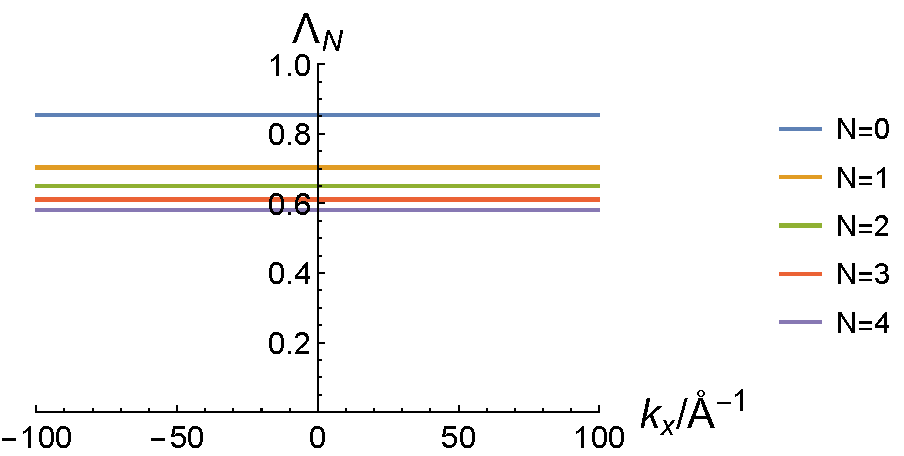
\includegraphics[scale=0.68]{figures/fig_3}
\caption{\label{fig_3} The dependence of normalized scattering-induced broadening $\Lambda_N$ for each Landau level ($N =0,1,2,3,4$) against $x$-directional momentum value $k_x$ in a GaAs-based quantum well at a magnetic field $B = 1.2~\text{T}$, dressing field with frequency $\omega =2\times10^{12}~\text{rad}\text{s}^{-1}$ and intensity $I =100~\text{W}/\text{cm}^{2}$. In this calculation we have assumed that the natural  broadening of $0$-th Landau level $\Gamma_0$ is $0.24\;\text{me}V$.}
\end{figure}
\begin{figure}[t]
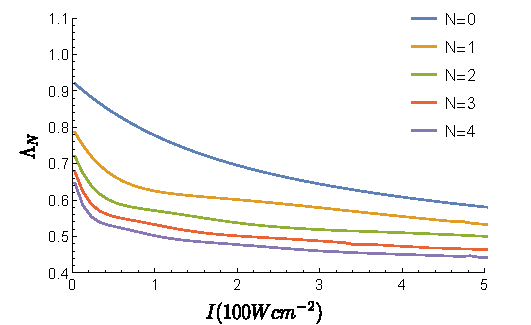
\includegraphics[scale=0.68]{figures/fig_4}
\caption{\label{fig_4} The dependence of normalized scattering-induced broadening $\Lambda_N$ for each Landau level ($N =0,1,2,3,4$) against dressing field intensity $I$, in a GaAs-based quantum well at a magnetic field $B = 1.2~\text{T}$, dressing field with frequency $\omega =2\times10^{12}~\text{rad}\text{s}^{-1}$. In this calculation we have assumed that the natural broadening of $0$-th Landau level $\Gamma_0$ is $0.24\;\text{me}V$.}
\end{figure}
